\documentclass[14pt]{beamer}

\title[Codiac]{Codiac}
\author[]{Coding Assistant for Beginners}
\date []{August - September, 2020}


\usetheme{Madrid}
\usecolortheme{beaver}
\usepackage[11pt]{moresize}
\usepackage{setspace}
\usepackage{hyperref}
\usepackage{graphicx}
\usepackage{caption}
\usepackage{subcaption}
\definecolor{dr}{rgb}{30, 0, 0}

\begin{document}

\begin{frame}
    \noindent
    {\color{pink} \rule{\linewidth}{0.7mm} }
    \titlepage
    \noindent
    {\color{pink} \rule{\linewidth}{0.7mm} }
\end{frame}

\begin{frame}
    \frametitle{About Us}
    \noindent
    {\color{pink} \rule {\linewidth}{0.7mm}}
    \begin{itemize}
      \item [] 
\includegraphics[width=1in, height=1in]{./Codiac/logos/rushali.jpeg}\hspace{1cm} 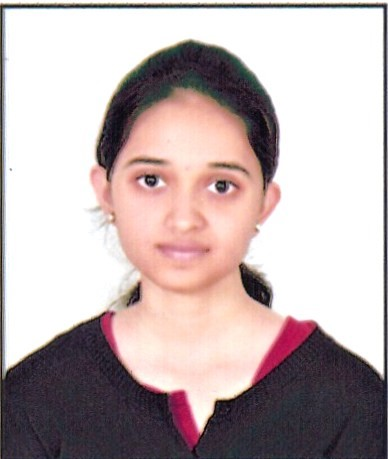
\includegraphics[width=1in, height=1in]{./Codiac/logos/sudha.jpeg}\hspace{1cm} 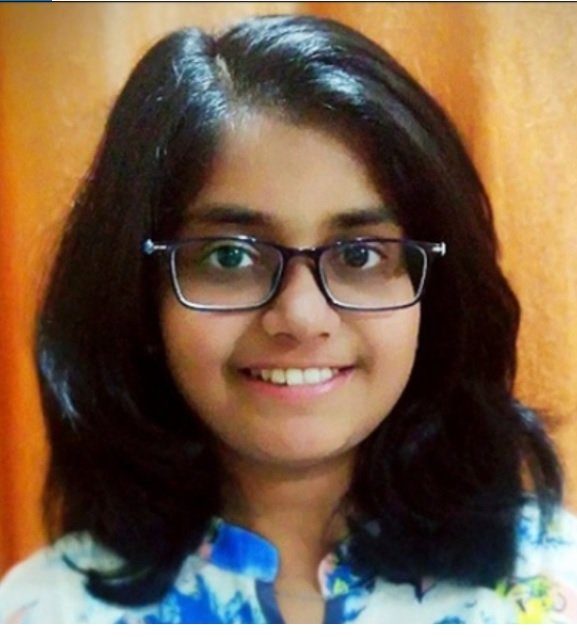
\includegraphics[width=1in, height=1in]{./Codiac/logos/nimisha.jpg}\hspace{1cm} \\
      \item [] Rushali\hspace{2cm} Sai Sudha\hspace{1.8cm} Nimisha\\
      \item [] \small CGEC\hspace{2.5cm} \small GPREC \hspace{2.4cm} \small VU\\
      \item [] \small CoochBehar\hspace{1.5cm} \small Kurnool \hspace{2.2cm} \small Pune\\
    \end{itemize}
    \noindent
    {\color{pink} \rule{\linewidth}{0.7mm}}
\end{frame}



\begin{frame}
    \frametitle{Why Codiac?}
    \noindent
    {\color{pink} \rule{\linewidth}{0.7mm} }
    \begin{itemize}
    \item [$\bigstar$] Lack of Beginner level Assistance \\
    \item [$\bigstar$] Too many Resources creating Confusions \\  
   \item [$\bigstar$] Interactive Learning \\
    \end{itemize}
    \noindent
     {\color{pink} \rule{\linewidth}{0.7mm}}
\end{frame}


\begin{frame}
\frametitle{Overview}
\noindent
{\color{pink} \rule{\linewidth}{0.7mm} }
     \begin{figure}[htbp]
      \centerline{
\includegraphics[width=2.3in, height=1.3in]{./Codiac/logos/logo.jpeg}}
     \end{figure}
\small ``Codiac'' is your one stop destination to start learning to code. From answering your queries to teaching you just from scratch, well you got everything you need as a beginner here!
\noindent
{\color{pink} \rule{\linewidth}{0.7mm} } 
\end{frame}   

\begin{frame}
     \frametitle{Survey}
     \begin{figure}[htbp]
         \centerline{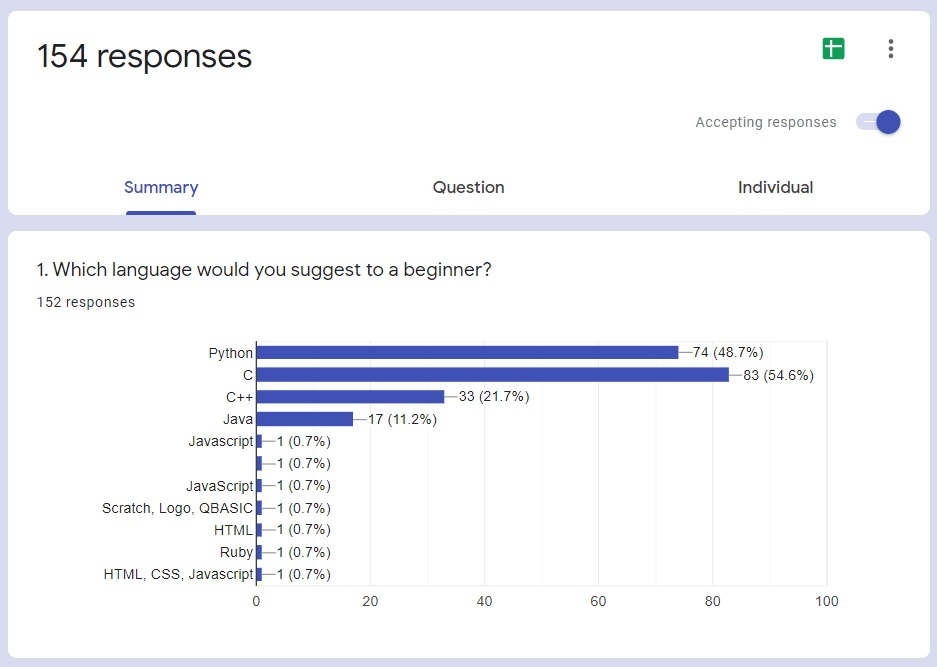
\includegraphics[width=4in, height=3in]{./Codiac/logos/form.jpeg}}
         \begin{spacing}{0.25}
         \end{spacing}
     \end{figure}
 \end{frame}




\begin{frame}
    \frametitle{What we Offer?}
    \noindent
     {\color{pink} \rule{\linewidth}{1mm} }
    \begin{itemize}
        \item [] 
\includegraphics[width=0.5in, height=0.5in]{./Codiac/logos/c.png}\hspace{1cm}{\huge C} \\
          
        \item [] 
\includegraphics[width=0.5in, height=0.5in]{./Codiac/logos/python.png}\hspace{1cm}{\huge Python} \\
          
       \item [] 
\includegraphics[width=0.5in, height=0.5in]{./Codiac/logos/bot.jpg}\hspace{1cm}{\huge Bot} \\
          
      \item [] 
\includegraphics[width=0.5in, height=0.5in]{./Codiac/logos/forum.png}\hspace{1cm}{\huge Discussion Forum} \\
    \end{itemize}
\noindent
    {\color{pink} \rule{\linewidth}{1mm} }
\end{frame}

   

\begin{frame}
    \frametitle{Technology Stack}
    \noindent
    {\color{pink} \rule{\linewidth}{0.7mm} }
    \begin{itemize}
        \item [] 
\includegraphics[width=0.2in, height=0.2in]{./Codiac/logos/html.png} HTML5 \\
            
        \item [] 
\includegraphics[width=0.2in, height=0.2in]{./Codiac/logos/css.png} CSS3 \\
            
        \item [] 
\includegraphics[width=0.2in, height=0.2in]{./Codiac/logos/java.png} Javascript \\
            
        \item [] 
\includegraphics[width=0.2in, height=0.2in]{./Codiac/logos/w3.png} W3.CSS \\
            
        \item [] 
\includegraphics[width=0.2in, height=0.2in]{./Codiac/logos/flask.jpg} Flask \\
            
        \item [] 
\includegraphics[width=0.2in, height=0.2in]{./Codiac/logos/sqllite.png} SQLite \\
            
        \item [] 
\includegraphics[width=0.2in, height=0.2in]{./Codiac/logos/dialogflow.jpg} Dialogflow \\
            
        \item [] 
\includegraphics[width=0.2in, height=0.2in]{./Codiac/logos/git.png} Git \\
            
        \item [] 
\includegraphics[width=0.2in, height=0.2in]{./Codiac/logos/latex.png} LaTeX \\
    \end{itemize}
\noindent
    {\color{pink} \rule{\linewidth}{0.7mm} }
\end{frame}

\begin{frame}
    \frametitle{Learnings}
    \noindent
    {\color{pink} \rule{\linewidth}{0.7mm} }
    \begin{itemize}
    \item [] 
\includegraphics[width=0.2in, height=0.2in]{./Codiac/logos/check.png} Front End Development \\
        
    \item [] 
\includegraphics[width=0.2in, height=0.2in]{./Codiac/logos/check.png} Back End Development \\
        
    \item [] 
\includegraphics[width=0.2in, height=0.2in]{./Codiac/logos/check.png} Database\\
        
   \item [] 
\includegraphics[width=0.2in, height=0.2in]{./Codiac/logos/check.png} Version Control \\

   \item [] 
\includegraphics[width=0.2in, height=0.2in]{./Codiac/logos/check.png} LaTeX \\
  
\end{itemize}
\noindent
    {\color{pink} \rule{\linewidth}{0.7mm} }
\end{frame}


\begin{frame}
      \frametitle{Statistics}
        \begin{figure}[htbp]
        \centerline{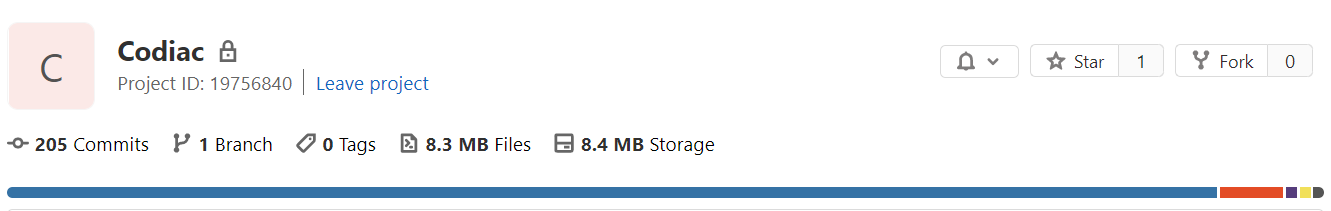
\includegraphics[width=4in, height=1in]{./Codiac/logos/commits.png}}
  \end{figure}
\end{frame}


\begin{frame}
    \frametitle{Challenges}
    \noindent
    {\color{pink} \rule{\linewidth}{0.7mm} }
    \begin{itemize}
    \item [] 
\includegraphics[width=0.2in, height=0.2in]{./Codiac/logos/exclamation.png} Bot Integration\\
        
    \item [] 
\includegraphics[width=0.2in, height=0.2in]{./Codiac/logos/exclamation.png} Screening Content\\
                
    \item [] 
\includegraphics[width=0.2in, height=0.2in]{./Codiac/logos/exclamation.png} Appearance\\
            \item [] 
\includegraphics[width=0.2in, height=0.2in]{./Codiac/logos/exclamation.png} Discussion Forum\\
\end{itemize}
\noindent
    {\color{pink} \rule{\linewidth}{0.7mm} }
\end{frame}

\begin{frame}
     \frametitle{Demo}
       {\color{dr} \rule{\linewidth}{0.7mm}}
       \linebreak
        \linebreak
        \centerline
        {\huge \color{dr}
        \href{https://codiac-codenow.herokuapp.com}{Let's Code with Codiac !}}
        \linebreak
     {\color{dr} \rule{\linewidth}{0.7mm}}
  \end{frame}


\begin{frame}
    \frametitle{Future Scope}
	\noindent
    {\color{pink} \rule{\linewidth}{0.7mm}} 
         \begin{itemize}
 \item [] 
\includegraphics[width=0.3in, height=0.3in]{./Codiac/logos/loading.jpg} Languages on the way\\
     
 \item [] 
\includegraphics[width=0.3in, height=0.3in]{./Codiac/logos/loading.jpg} Personalized Experience \\
 \end{itemize}
\noindent{	
	   \color{pink} \rule{\linewidth}{0.7mm} }   	
\end{frame}	


\begin{frame}
	\frametitle{References}
    \noindent
    {\color{pink} \rule{\linewidth}{0.7mm}}
    \begin{itemize}
        \item [] 
\includegraphics[width=0.3in, height=0.3in]{./Codiac/logos/documentation.png} \href{https://flask.palletsprojects.com/en/1.1.x/} {Flask Documentation}\\
            
        \item [] 
\includegraphics[width=0.3in, height=0.3in]{./Codiac/logos/w3schools.png} \href{https://www.w3schools.com/} {W3 Schools Website}\\
            \item [] 
\includegraphics[width=0.3in, height=0.3in]{./Codiac/logos/botcopy.png} \href{https://www.botcopy.com/} {Bot Copy and Janis}\\
                    \item [] 
\includegraphics[width=0.3in, height=0.3in]{./Codiac/logos/shutter.png} \href{https://www.shutterstock.com/?rid=170336628&gclid=Cj0KCQjwnqH7BRDdARIsACTSAdvbnRVMWw3_B9aDsAxuGgPnMgjnuE9Gdei2Z510VfgXOn-pviSB-YMaAv6vEALw_wcB} {Shutterstock}\\
                    \item [] 
\includegraphics[width=0.3in, height=0.3in]{./Codiac/logos/heroku.jpg} \href{https://signup.heroku.com/t/platform?c=7013A000000ib1xQAA&gclid=CjwKCAjwh7H7BRBBEiwAPXjadvVFuTYB80whEdGEBINmJF2RsYPX9X7iwQU11dya8QJAOFCxENHdrRoCiaMQAvD_BwE}{Heroku}\\
                     \item [] 
\includegraphics[width=0.3in, height=0.3in]{./Codiac/logos/gitlab.png} \href{https://gitlab.com/ksaisudha24/Codiac}{Link to our repository}\\
    \end{itemize}
    \noindent
    {\color{pink} \rule{\linewidth}{0.7mm}}
\end{frame}

\end{document}

